\section{Gram\'atica simple}

Despu\'es de revisar el an\'alisis del lenguaje natural, el resultado lo podemos expresar mediante un \'arbol. Los \'arboles son formas gr\'aficas que utilizaremos para expresar la estructura de la oraci\'on. \cite{elprofesionaldelainformacion}

	\begin{figure}[htbp!]
		\centering
			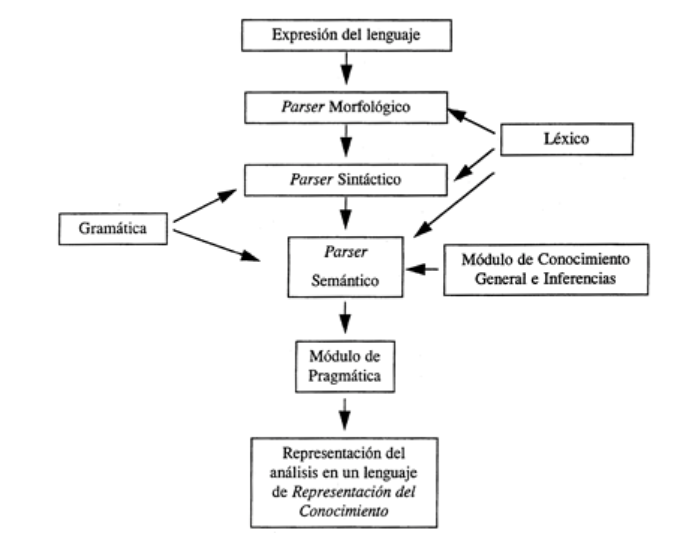
\includegraphics[width=0.8\textwidth]{images/gramatica}
		\caption{Gram\'atica simple}
	\end{figure}
	